% Created by tikzDevice version 0.12.6 on 2024-08-06 17:34:23
% !TEX encoding = UTF-8 Unicode
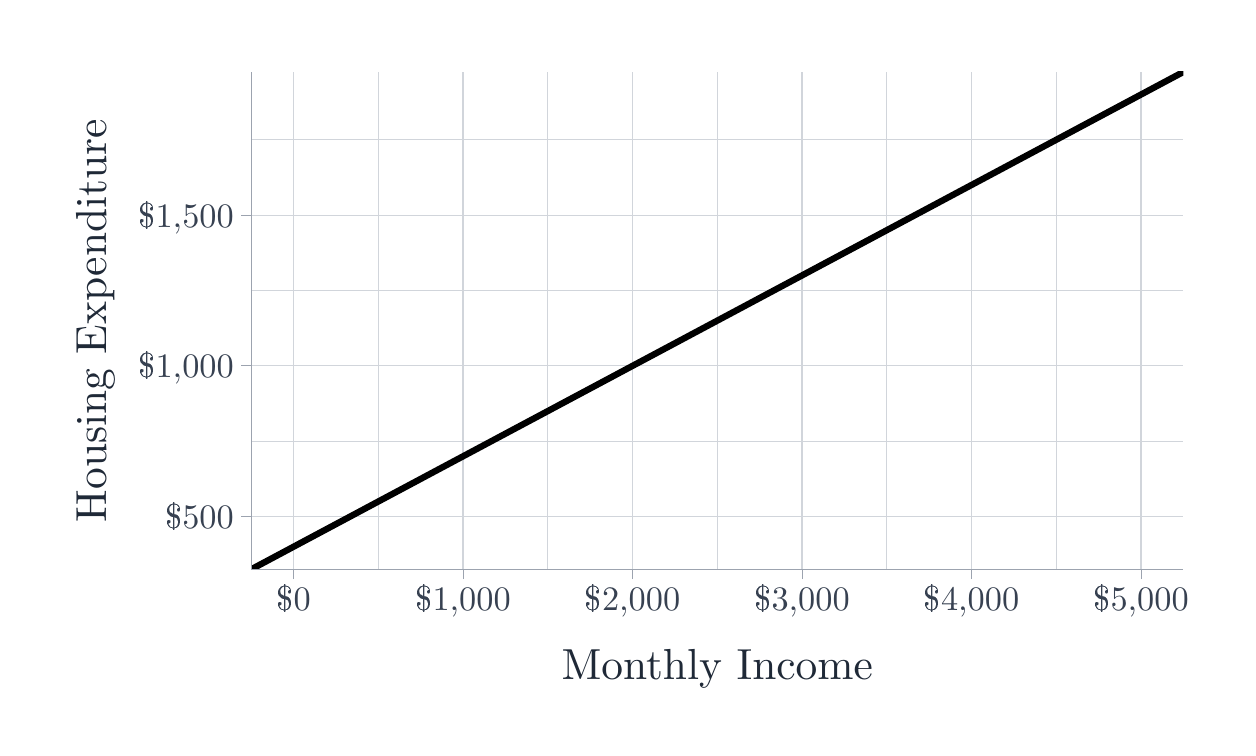
\begin{tikzpicture}[x=1pt,y=1pt]
\definecolor{fillColor}{RGB}{255,255,255}
\path[use as bounding box,fill=fillColor] (0,0) rectangle (433.62,252.94);
\begin{scope}
\path[clip] (  0.00,  0.00) rectangle (433.62,252.94);
\definecolor{drawColor}{RGB}{255,255,255}

\path[draw=drawColor,line width= 0.7pt,line join=round,line cap=round,fill=fillColor] (  0.00,  0.00) rectangle (433.62,252.94);
\end{scope}
\begin{scope}
\path[clip] ( 80.76, 57.20) rectangle (417.62,236.94);
\definecolor{drawColor}{RGB}{255,255,255}
\definecolor{fillColor}{RGB}{255,255,255}

\path[draw=drawColor,line width= 0.7pt,line join=round,line cap=round,fill=fillColor] ( 80.76, 57.20) rectangle (417.62,236.94);
\definecolor{drawColor}{RGB}{209,213,219}

\path[draw=drawColor,line width= 0.4pt,line join=round] ( 80.76,103.49) --
	(417.62,103.49);

\path[draw=drawColor,line width= 0.4pt,line join=round] ( 80.76,157.96) --
	(417.62,157.96);

\path[draw=drawColor,line width= 0.4pt,line join=round] ( 80.76,212.43) --
	(417.62,212.43);

\path[draw=drawColor,line width= 0.4pt,line join=round] (126.69, 57.20) --
	(126.69,236.94);

\path[draw=drawColor,line width= 0.4pt,line join=round] (187.94, 57.20) --
	(187.94,236.94);

\path[draw=drawColor,line width= 0.4pt,line join=round] (249.19, 57.20) --
	(249.19,236.94);

\path[draw=drawColor,line width= 0.4pt,line join=round] (310.44, 57.20) --
	(310.44,236.94);

\path[draw=drawColor,line width= 0.4pt,line join=round] (371.68, 57.20) --
	(371.68,236.94);

\path[draw=drawColor,line width= 0.4pt,line join=round] ( 80.76, 76.26) --
	(417.62, 76.26);

\path[draw=drawColor,line width= 0.4pt,line join=round] ( 80.76,130.73) --
	(417.62,130.73);

\path[draw=drawColor,line width= 0.4pt,line join=round] ( 80.76,185.20) --
	(417.62,185.20);

\path[draw=drawColor,line width= 0.4pt,line join=round] ( 96.07, 57.20) --
	( 96.07,236.94);

\path[draw=drawColor,line width= 0.4pt,line join=round] (157.32, 57.20) --
	(157.32,236.94);

\path[draw=drawColor,line width= 0.4pt,line join=round] (218.56, 57.20) --
	(218.56,236.94);

\path[draw=drawColor,line width= 0.4pt,line join=round] (279.81, 57.20) --
	(279.81,236.94);

\path[draw=drawColor,line width= 0.4pt,line join=round] (341.06, 57.20) --
	(341.06,236.94);

\path[draw=drawColor,line width= 0.4pt,line join=round] (402.31, 57.20) --
	(402.31,236.94);
\definecolor{drawColor}{RGB}{0,0,0}

\path[draw=drawColor,line width= 2.3pt,line join=round] (-256.11,-122.55) -- (754.48,416.69);
\end{scope}
\begin{scope}
\path[clip] (  0.00,  0.00) rectangle (433.62,252.94);
\definecolor{drawColor}{RGB}{156,163,175}

\path[draw=drawColor,line width= 0.3pt,line join=round] ( 80.76, 57.20) --
	( 80.76,236.94);
\end{scope}
\begin{scope}
\path[clip] (  0.00,  0.00) rectangle (433.62,252.94);
\definecolor{drawColor}{RGB}{55,65,81}

\node[text=drawColor,anchor=base east,inner sep=0pt, outer sep=0pt, scale=  1.24] at ( 74.46, 71.98) {\$500};

\node[text=drawColor,anchor=base east,inner sep=0pt, outer sep=0pt, scale=  1.24] at ( 74.46,126.45) {\$1,000};

\node[text=drawColor,anchor=base east,inner sep=0pt, outer sep=0pt, scale=  1.24] at ( 74.46,180.91) {\$1,500};
\end{scope}
\begin{scope}
\path[clip] (  0.00,  0.00) rectangle (433.62,252.94);
\definecolor{drawColor}{RGB}{156,163,175}

\path[draw=drawColor,line width= 0.3pt,line join=round] ( 77.26, 76.26) --
	( 80.76, 76.26);

\path[draw=drawColor,line width= 0.3pt,line join=round] ( 77.26,130.73) --
	( 80.76,130.73);

\path[draw=drawColor,line width= 0.3pt,line join=round] ( 77.26,185.20) --
	( 80.76,185.20);
\end{scope}
\begin{scope}
\path[clip] (  0.00,  0.00) rectangle (433.62,252.94);
\definecolor{drawColor}{RGB}{156,163,175}

\path[draw=drawColor,line width= 0.3pt,line join=round] ( 80.76, 57.20) --
	(417.62, 57.20);
\end{scope}
\begin{scope}
\path[clip] (  0.00,  0.00) rectangle (433.62,252.94);
\definecolor{drawColor}{RGB}{156,163,175}

\path[draw=drawColor,line width= 0.3pt,line join=round] ( 96.07, 53.70) --
	( 96.07, 57.20);

\path[draw=drawColor,line width= 0.3pt,line join=round] (157.32, 53.70) --
	(157.32, 57.20);

\path[draw=drawColor,line width= 0.3pt,line join=round] (218.56, 53.70) --
	(218.56, 57.20);

\path[draw=drawColor,line width= 0.3pt,line join=round] (279.81, 53.70) --
	(279.81, 57.20);

\path[draw=drawColor,line width= 0.3pt,line join=round] (341.06, 53.70) --
	(341.06, 57.20);

\path[draw=drawColor,line width= 0.3pt,line join=round] (402.31, 53.70) --
	(402.31, 57.20);
\end{scope}
\begin{scope}
\path[clip] (  0.00,  0.00) rectangle (433.62,252.94);
\definecolor{drawColor}{RGB}{55,65,81}

\node[text=drawColor,anchor=base,inner sep=0pt, outer sep=0pt, scale=  1.24] at ( 96.07, 42.33) {\$0};

\node[text=drawColor,anchor=base,inner sep=0pt, outer sep=0pt, scale=  1.24] at (157.32, 42.33) {\$1,000};

\node[text=drawColor,anchor=base,inner sep=0pt, outer sep=0pt, scale=  1.24] at (218.56, 42.33) {\$2,000};

\node[text=drawColor,anchor=base,inner sep=0pt, outer sep=0pt, scale=  1.24] at (279.81, 42.33) {\$3,000};

\node[text=drawColor,anchor=base,inner sep=0pt, outer sep=0pt, scale=  1.24] at (341.06, 42.33) {\$4,000};

\node[text=drawColor,anchor=base,inner sep=0pt, outer sep=0pt, scale=  1.24] at (402.31, 42.33) {\$5,000};
\end{scope}
\begin{scope}
\path[clip] (  0.00,  0.00) rectangle (433.62,252.94);
\definecolor{drawColor}{RGB}{31,41,55}

\node[text=drawColor,anchor=base,inner sep=0pt, outer sep=0pt, scale=  1.57] at (249.19, 17.53) {Monthly Income};
\end{scope}
\begin{scope}
\path[clip] (  0.00,  0.00) rectangle (433.62,252.94);
\definecolor{drawColor}{RGB}{31,41,55}

\node[text=drawColor,rotate= 90.00,anchor=base,inner sep=0pt, outer sep=0pt, scale=  1.57] at ( 28.38,147.07) {Housing Expenditure};
\end{scope}
\end{tikzpicture}
